\documentclass[12pt, letterpaper]{article}

\usepackage[english]{babel} % Sets the language and regional settings for English documents
\usepackage[utf8]{inputenc} % Allows the use of UTF-8 characters in the document
\usepackage[T1]{fontenc} % Specifies the font encoding
\usepackage[margin=2cm]{geometry} % Sets the page margins
\usepackage{makeidx} % Enables the creation of indexes
\usepackage{natbib} % Provides flexible bibliography support
\usepackage{url} % Allows the use of URLs
\usepackage{enumitem} % Customizes the appearance of lists
\usepackage{listings} % Provides syntax highlighting for code listings
\usepackage[dvipsnames]{xcolor} % Allows the use of colors
\usepackage{parskip} % Modifies paragraph spacing
\usepackage{graphicx} % Enables the inclusion of graphics
\usepackage{tikz} % Allows the creation of graphics and diagrams
\usepackage{float}
\usepackage{hyperref} % Enables the creation of hyperlinks
\usepackage{amsmath} % Provides additional math environments and commands
\usepackage{circuitikz} % Allows the creation of electrical circuits
\usepackage{adjustbox} % Adjusts the size of the circuit diagrams
\usepackage{arydshln} % Allows the use of dashed lines in tables

\usetikzlibrary{shapes.geometric, positioning}

\lstset{
	language=SQL,
	basicstyle=\ttfamily\small,
	keywordstyle=\color{blue},
	commentstyle=\color[rgb]{0,0.5,0},
	stringstyle=\color{red},
	numbers=left,
	numberstyle=\tiny\color{gray},
	stepnumber=1,
	numbersep=10pt,
	backgroundcolor=\color{white},
	showspaces=false,
	showstringspaces=false,
	breaklines=true,
	frame=single,
	tabsize=2, captionpos=b, lineskip=-1pt,
	extendedchars=true,
	literate={á}{{\'a}}1 {é}{{\'e}}1 {í}{{\'i}}1 {ó}{{\'o}}1 {ú}{{\'u}}1 {Á}{{\'A}}1 {É}{{\'E}}1 {Í}{{\'I}}1 {Ó}{{\'O}}1 {Ú}{{\'U}}1 {ñ}{{\~n}}1 {Ñ}{{\~N}}1 {¿}{{\textquestiondown}}1 {¡}{{\textexclamdown}}1
}

\graphicspath{ {./img/} } % Sets the path for the graphics

\newlist{biblio}{enumerate}{1}
\setlist[biblio,1]{label=[\arabic*]}

\makeindex

\begin{document}

\begin{titlepage}

	\begin{tikzpicture}[remember picture,overlay]
		\node[anchor=north west, inner sep=30] at (current page.north west) {
			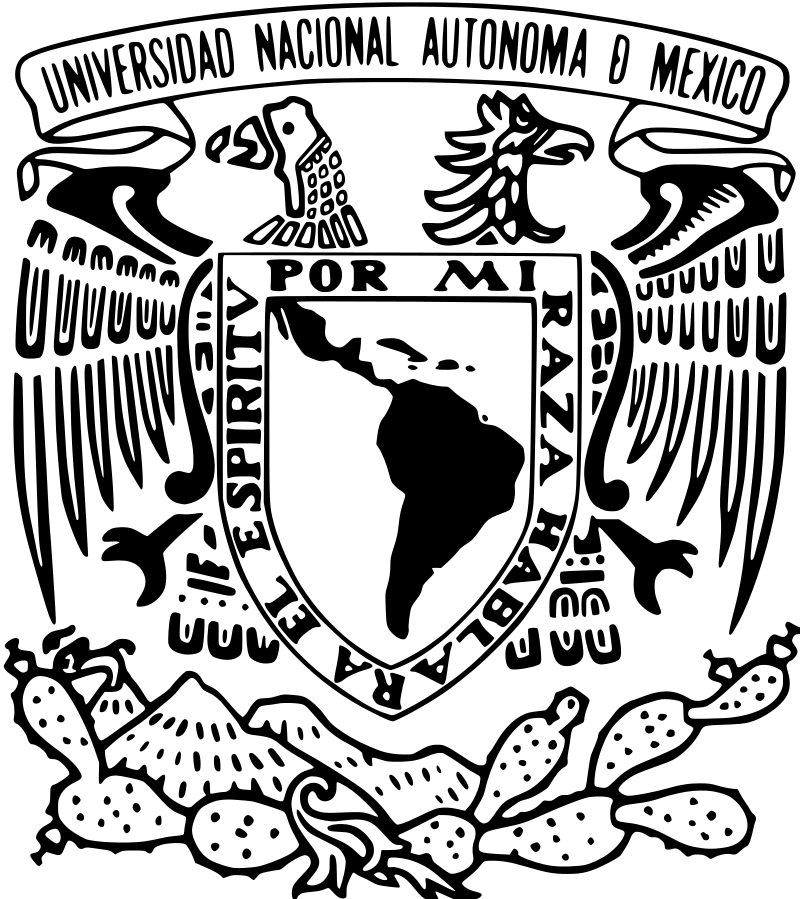
\includegraphics[width=4cm]{escudoUNAM.png}
		};

		\node[anchor=north east, inner sep=30] at (current page.north east) {
			
\includegraphics[width=4cm]{escudoFI.png}
		};
	\end{tikzpicture}

	\begin{center}
		\vspace*{3cm}

		\Huge
		\textbf{Práctica 1 - Sistemas Eléctricos de Primero y Segundo Orden}\\

		\vspace{2.5cm}

		\Huge
		\textbf{Facultad de Ingeniería}\\
		C		Semestre 2026-1\\

		\vspace{2.5cm}

		\textbf{Grupo:} 4

		\vspace{2.5cm}

		\Huge
		\textbf{Integrantes brigada 6:}\\
		Ugartechea González Luis Antonio 320223822\\
		Tepal Briseño Hansel Yael 320078282\\
		\vspace{2.5cm}
		\textbf{Fecha de entrega:} 02 de septiembre de 2025\\
	\end{center}
\end{titlepage}

\section{Objetivo}

Realizar mediciones de la constante de tiempo de circuitos de primer orden y los parámetros de diseño de un circuito de segundo orden; mediante la respuesta a escalón.

\section{Introducción}

En esta práctica vamos a ver cómo los circuitos eléctricos de primer y segundo orden responden cuando les aplicamos diferentes señales. Usamos la transformada de Laplace para entender mejor lo que pasa y sacar la función de transferencia, que nos ayuda a ver la relación entre la entrada y la salida. Además, medimos cosas como la constante de tiempo y el factor de amortiguamiento para entender cómo afectan la respuesta de los circuitos en situaciones reales.

\section{Desarrollo}

\subsection{Experimento 1: Medición de Inductancia}

Una vez armado el circuito de la figura \ref{fig:circuito_inductancia} determinamos experimentalmente la constante del tiempo \(\tau\).

\begin{figure}[H]
	\centering
	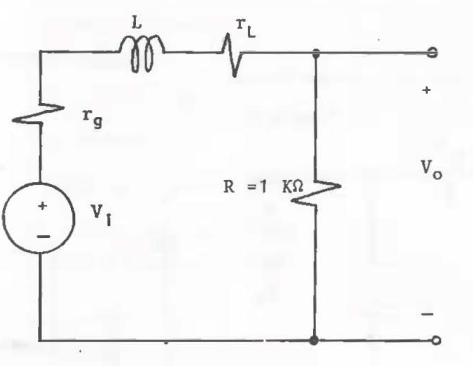
\includegraphics[width=0.6\textwidth]{circuito_1.png}
	\caption{Circuito para medición de inductancia}
	\label{fig:circuito_inductancia}
\end{figure}

Datos del circuito:

\begin{itemize}
	\item \(r_g = 50 \Omega\)
	\item \(L = 72 mH\)
	\item \(R_L = 72.7 \Omega\)
	\item \(R = 1000 \Omega\)
	\item  \(F = 1000 Hz\)
	\item \(V_{in} = 10 V_{pp}\)
\end{itemize}

Antes de comparar con el valor experimental, obtuvimos el valor teórico de la constante de tiempo \(\tau\) para el circuito RL, para así poder medir el porcentaje de error experimental que obtuvimos al realizar nuestras mediciones con respecto al valor de la inductancia.

La constante de tiempo \(\tau\) para un circuito RL se calcula con la fórmula:

\[\tau_t = \frac{L}{R_{eq}}\]

Sustituyendo los valores dados:

\[\tau_t = \frac{72 mH}{50 \Omega + 72.7 \Omega + 1000 \Omega}\]

\[\tau_t = 64.159 \, \mu s\]

\subsubsection{Resultados del osciloscopio}

\begin{figure}[H]
	\centering
	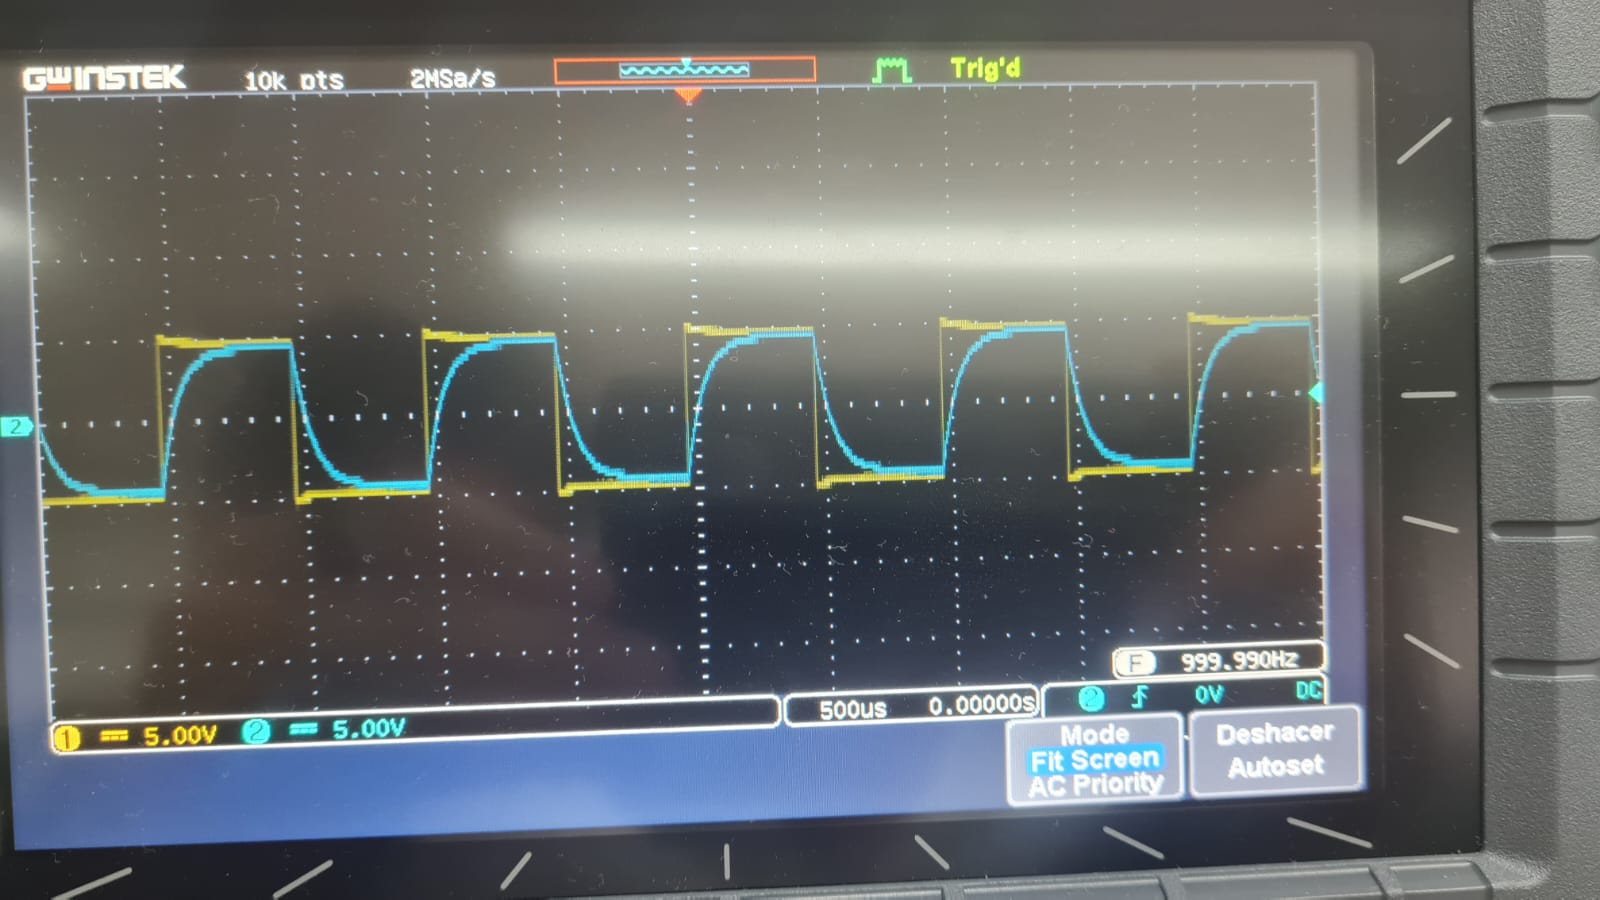
\includegraphics[width=0.5\textwidth]{ejercicio_1.jpeg}
	\caption{Resultados del osciloscopio para la medición de inductancia}
	\label{fig:Osciloscopio_Inductancia}
\end{figure}

Experimentalmente se obtuvo una \(\tau\) de:

\(\tau_e = 68 \, \mu s\).

Despejando la inductancia \(L\) tenemos:

\[L = \tau \cdot R_{eq}\]

Sustituyendo los valores:

\[L = 68 \, \mu s \cdot (50 \Omega + 72.7 \Omega + 1000 \Omega)\]

\[L = 68 \, \mu s \cdot 1122.7 \Omega\]

\[L = 76.3 \, mH\]

Para calcular el porcentaje de error entre el valor teórico y el valor experimental usamos la siguiente fórmula:

\[ \text{Porcentaje de error} = \left| \frac{\text{Valor teórico} - \text{Valor experimental}}{\text{Valor teórico}} \right| \times 100\% \]

Sustituyendo los valores:

\[ \text{Porcentaje de error} = \left| \frac{76.3 \, mH - 72 \, mH}{76.3 \, mH} \right| \times 100\% \]

\[ \text{Porcentaje de error} = 5.63\% \]

\subsection{Experimento 2: Medición de Capacitancia}

Armanos el circuito de la figura \ref{fig:circuito_capacitancia} y determinamos experimentalmente la constante del tiempo \(\tau\).

\begin{figure}[H]
	\centering
	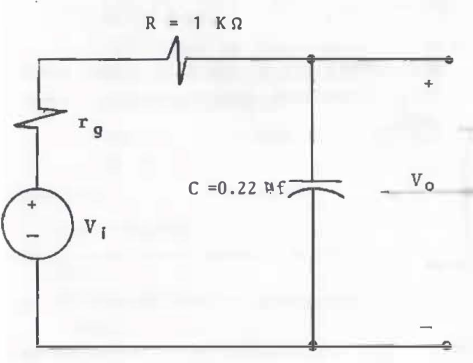
\includegraphics[width=0.6\textwidth]{circuito_2.png}
	\caption{Circuito para medición de inductancia}
	\label{fig:circuito_capacitancia}
\end{figure}

Datos del circuito:

\begin{itemize}
	\item \(r_g = 50 \Omega\)
	\item \(C = 0.22 \mu F\)
	\item \(R = 1000 \Omega\)
	\item  \(F = 500 Hz\)
	\item \(V_{in} = 10 V_{pp}\)
\end{itemize}

Antes de hacer nuestras mediciones con el osciloscopio, es importante calcular el valor teórico de la constante de tiempo \(\tau\) para el circuito RC para que de esta manera podamos medir el porcentaje de error experimental que obtuvimos al ralizar nuestras mediciones. 
La constante de tiempo \(\tau\) para un circuito RC se calcula con la fórmula:

\[\tau_t = R \cdot C\]

Sustituyendo los valores dados:

\[\tau_t = 1050 \Omega \cdot 0.22 \mu F\]

\[\tau_t = 0.231 \mu s\]

\subsubsection{Resultados del osciloscopio}

\begin{figure}[H]
	\centering
	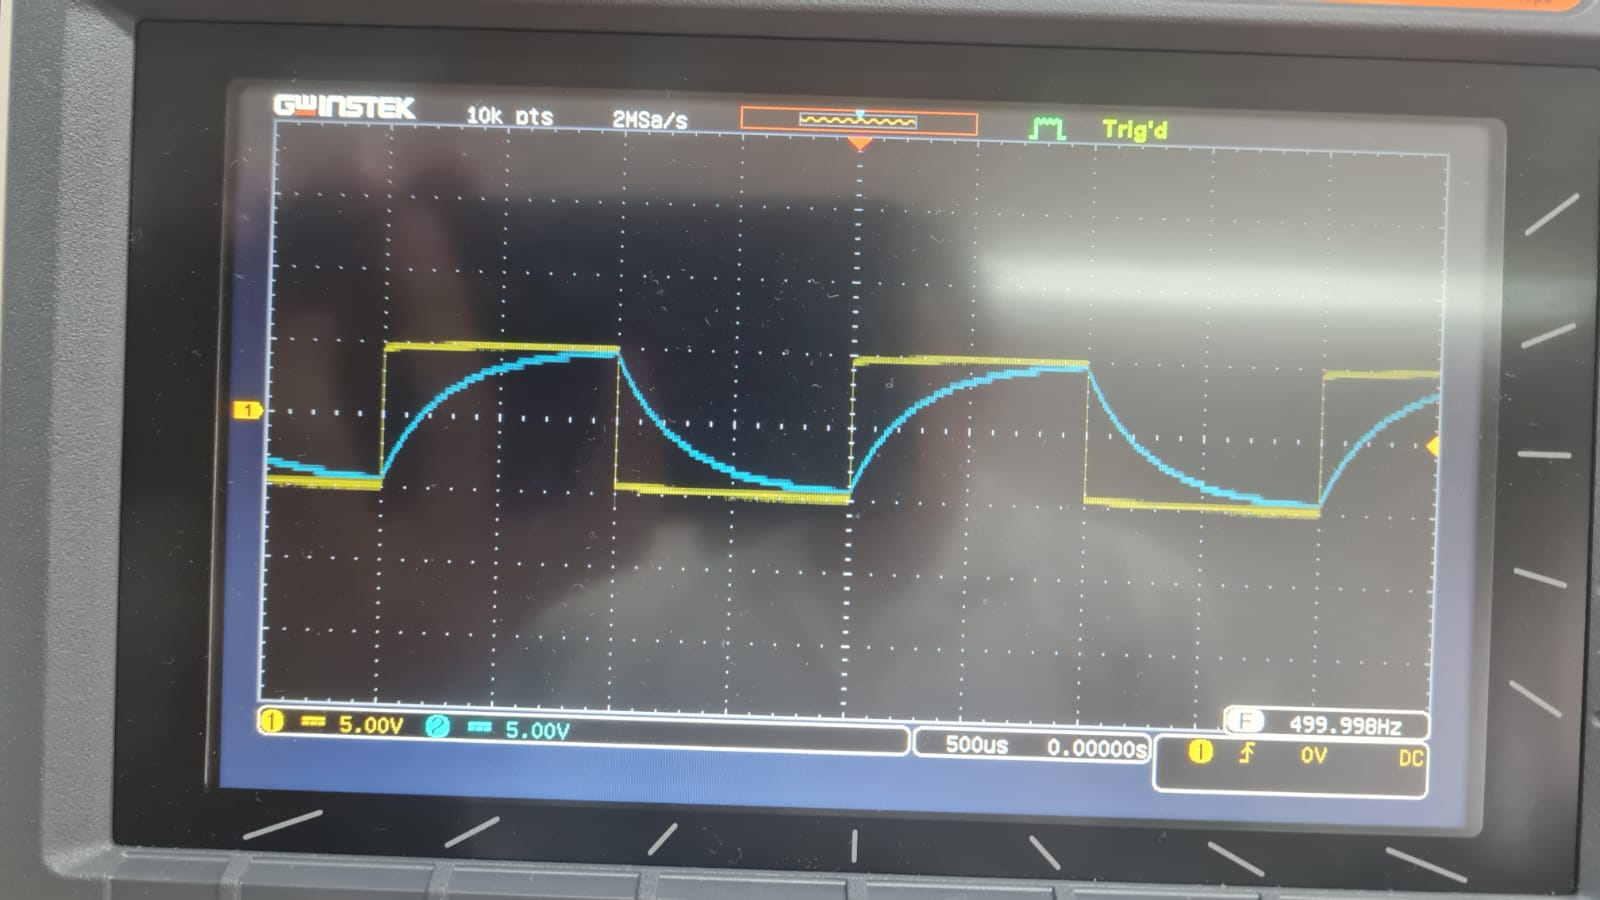
\includegraphics[width=0.5\textwidth]{ejercicio_2.jpeg}
	\caption{Circuito para medición de inductancia}
	\label{fig:Osciloscopio_Capacitancia}
\end{figure}

A partir de nuestras mediciones logramos determinar que el valor experimental que obtuvimos de nuestra constante de tiempo \(\tau_e\) era igual a \(242 \mu s\).

por lo que el valor experimental de nuestra capacitancia es:
\[C = \frac{\tau_e}{R}\]
\[C = \frac{242 \mu s}{1050 \Omega}\]
\[C = 0.23 \mu F\]

Para calcular el porcentaje de error entre el valor teórico y el valor experimental usamos la siguiente fórmula:

\[ \text{Porcentaje de error} = \left| \frac{\text{Valor teórico} - \text{Valor experimental}}{\text{Valor teórico}} \right| \times 100\% \]

Sustituyendo los valores:

\[ \text{Porcentaje de error} = \left| \frac{0.22 \mu F - 0.23 \mu F}{0.22 \mu F} \right| \times 100\% \]


\[ \text{Porcentaje de error} = 4.55\% \]

\subsection{Experimento 3: Sistema eléctrico de Segundo Orden}

\begin{figure}[H]
	\centering
	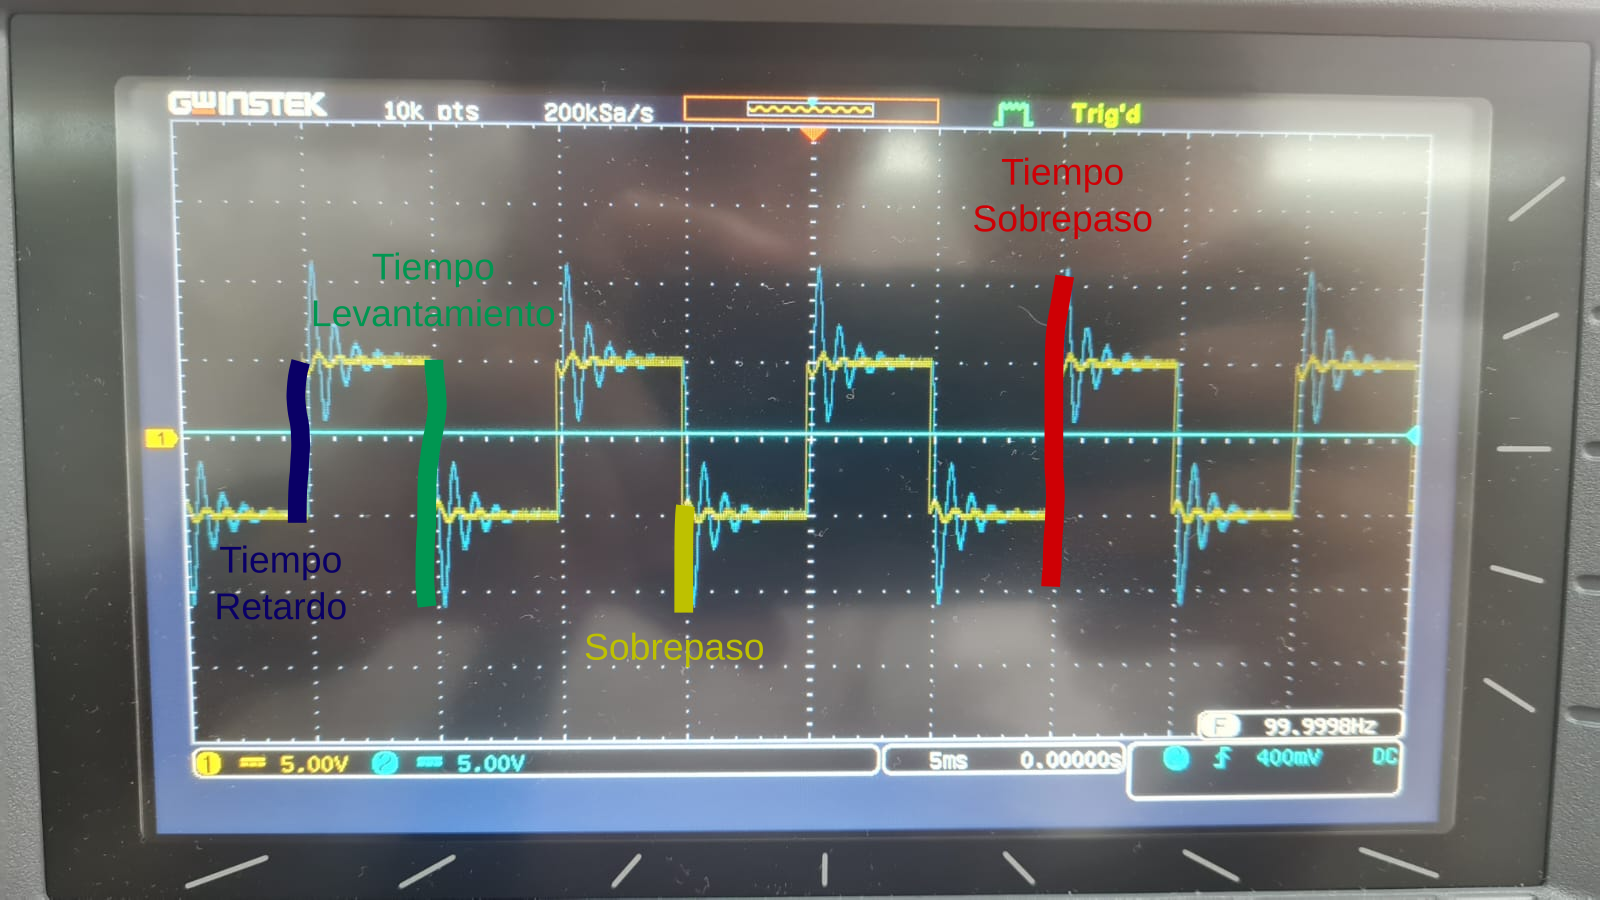
\includegraphics[width=0.8\textwidth]{ejercicio_3_1_edited.png}
	\caption{Circuito para medición de inductancia}
	\label{fig:Osciloscopio_RLC}
\end{figure}

\section{Conclusiones}

\subsection{Ugartechea González Luis Antonio}

Durante la práctica se alcanzaron los objetivos planteados, ya que se logró obtener experimentalmente la constante de tiempo \(\tau\), lo cual permitió comparar los resultados con los valores teóricos de los componentes \(L\) y \(C\). El error porcentual encontrado fue menor al $6\%$, lo que respalda la confiabilidad de los datos.

Además, el análisis de la respuesta a la señal escalón facilitó la identificación de los parámetros de diseño de un sistema de segundo orden, aunque el trabajo en el laboratorio quedó inconcluso debido a las restricciones de tiempo.

\subsubsection{Tepal Briseño Hansel Yael}

A partir de los experimentos realizados se puede concluir que los objetivos de la práctica fueron alcanzados, pues no solo se determinó con éxito el valor experimental de la constante de tiempo \(\tau\), así como de los elementos \textbf{L} y \textbf{C}, sino que también se reforzaron conceptos teóricos esenciales. Entre ellos destacan la transformada de Laplace y la función de transferencia, herramientas clave para el estudio y modelado de circuitos eléctricos.

Si bien el último experimento no pudo desarrollarse en su totalidad, se comprendieron los aspectos más relevantes de la dinámica de un sistema de segundo orden, lo cual contribuye a una mejor interpretación del comportamiento transitorio en este tipo de sistemas.
% \section{Bibliography}

% \begin{biblio}
% 	%for: https://www.poli.edu.co/blog/poliverso/diseno-digital-que-es
% 	\item \textit{Diseño digital: qué es y por qué es importante.} (2021, August 26). Poliverso. Retrieved October 16, 2024, from: \textcolor{blue}{\underline{\url{https://www.poli.edu.co/blog/poliverso/diseno-digital-que-es}}}
% 	%for: https://www.sky6cancun.com/marketing/diseno-grafico/diseno-digital-que-es-y-para-que-sirve/
% 	\item \textit{Diseño digital: qué es y para qué sirve.} (2021, August 26). Sky6Cancún. Retrieved October 16, 2024, from: \textcolor{blue}{\underline{\url{https://www.sky6cancun.com/marketing/diseno-grafico/}}}
% \end{biblio}

\end{document}
